%5_1.tex

実装した命令が正しく出力されるか,図\ref{fig:add_array_c}
に示した配列加算のプログラムを入力としてアセンブリコードの出力を行った.

\begin{figure}[tb]
    \centering
    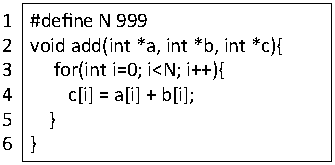
\includegraphics[scale=0.6]{image/add_array_c.pdf}
    \caption{配列加算プログラム}
    \label{fig:add_array_c}
\end{figure}

図\ref{fig:rv_vectorized_assembly}は
配列a,bの各要素の加算を配列cに格納する関数addのアセンブリコードで,データ数999個に対して一度にベクトル演算を行う配列要素を4として生成を行ったものである.25行目にあるベクトル加算のための`vadd.w'が今回実装した我々のベクトル拡張付きRISC-Vの命令である.その他の命令はRISC-Vで定義されている命令である.処理の流れはラベル`.LBB0\_2'にてベクトル演算を行っており,ラベル`LBB0\_4'にて余りの要素の処理を行っている.

\begin{figure}
    \centering
    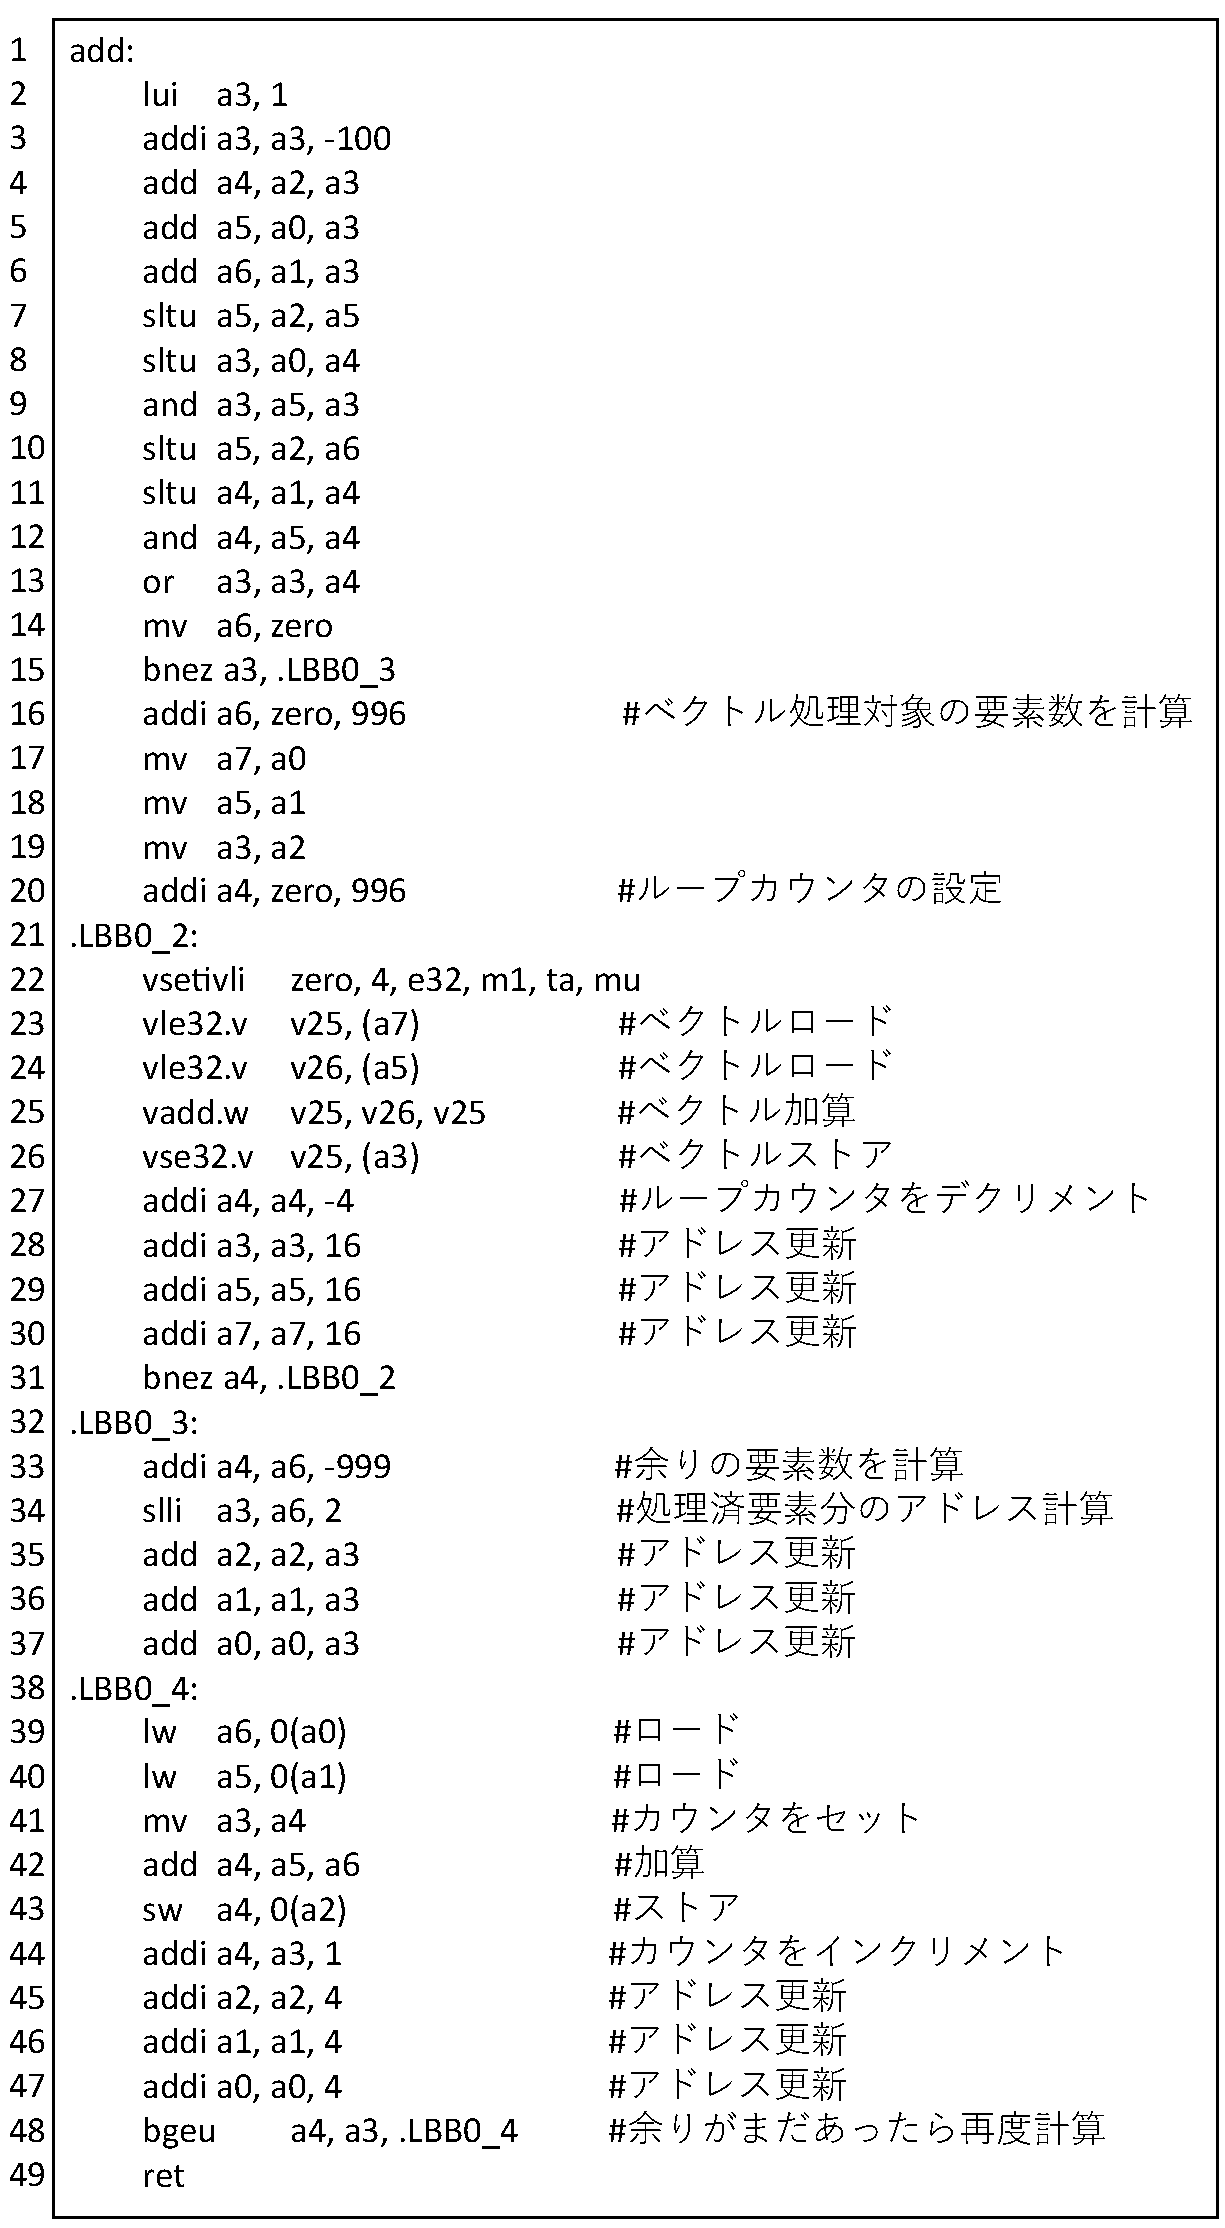
\includegraphics[scale=0.55]{image/rv_vectorized_assembly.pdf}
    \caption{生成されたアセンブリコード}
    \label{fig:rv_vectorized_assembly}
\end{figure}

図\ref{fig:add_array_c}の配列要素加算部分を変更し,他の定義した命令の生成を検証した.

ベクトル減算命令であるvsubの生成を図\ref{fig:vsub}
に,
ベクトル論理積,ベクトル論理和,ベクトル排他的論理和命令であるvand,vor,vxorの生成を図\ref{fig:vand},図\ref{fig:vor},図\ref{fig:vxor}に示す.

また,即値を用いたベクトル演算命令の生成も検証した.
即値によるベクトル加算・減算命令の生成を図に示す.定数を指定して配列要素への加算を行うプログラムを入力することで即値による加算命令となる.

同様に即値を用いる論理演算命令についてもvandiを図\ref{fig:vandi}
にvoriを図\ref{fig:vori}
にvxoriを図\ref{fig:vxori}
に示す.

即値によるベクトルシフト演算命令について,ベクトル論理左シフト命令であるvsllを図\ref{fig:vsll}
に示す.ベクトル算術右シフト命令であるvsraを図\ref{fig:vsra}
に示す.ベクトル論理右シフト命令であるvsrlを図\ref{fig:vsrl}
し示す.ベクトル論理右シフト命令を出力するためにC言語に変更を加えており,演算対象の配列の型宣言をint型からunsigned intに変更している.

\begin{figure}
    \centering
    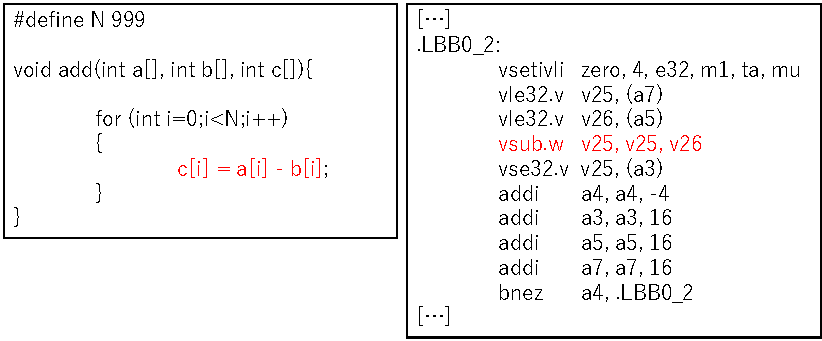
\includegraphics[scale=0.8]{image/vsub.pdf}
    \caption{vsub命令の生成}
    \label{fig:vsub}
\end{figure}

\begin{figure}
    \centering
    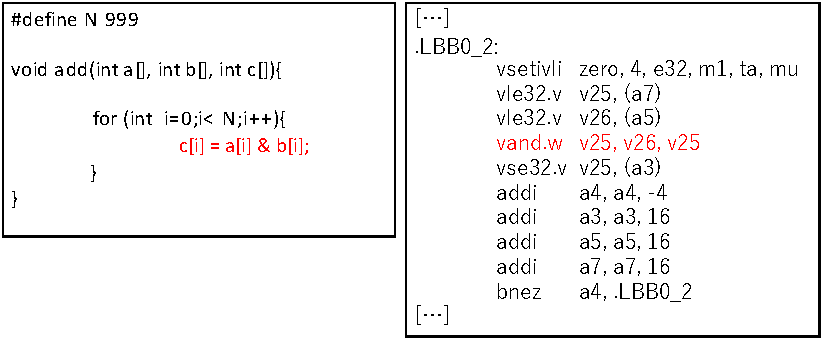
\includegraphics[scale=0.8]{image/vand.pdf}
    \caption{vand命令の生成}
    \label{fig:vand}
\end{figure}

\begin{figure}
    \centering
    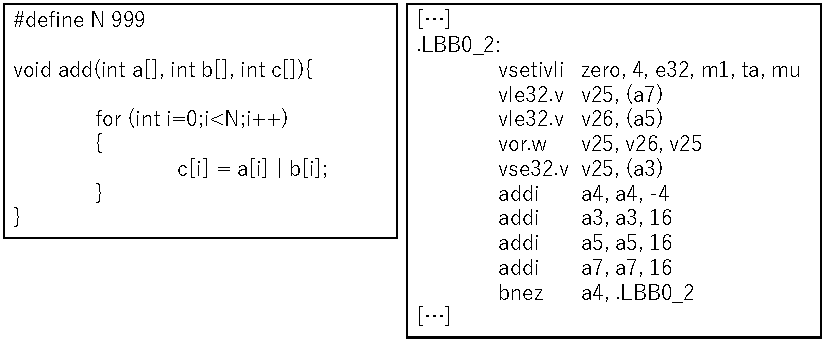
\includegraphics[scale=0.8]{image/vor.pdf}
    \caption{vor命令の生成}
    \label{fig:vor}
\end{figure}

\begin{figure}
    \centering
    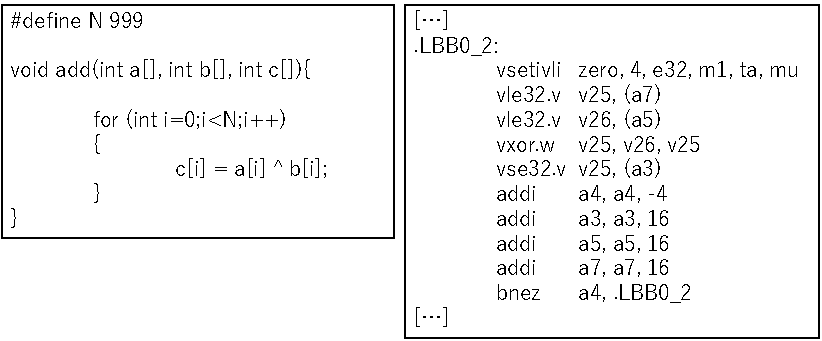
\includegraphics[scale=0.8]{image/vxor.pdf}
    \caption{vxor命令の生成}
    \label{fig:vxor}
\end{figure}

\begin{figure}
    \centering
    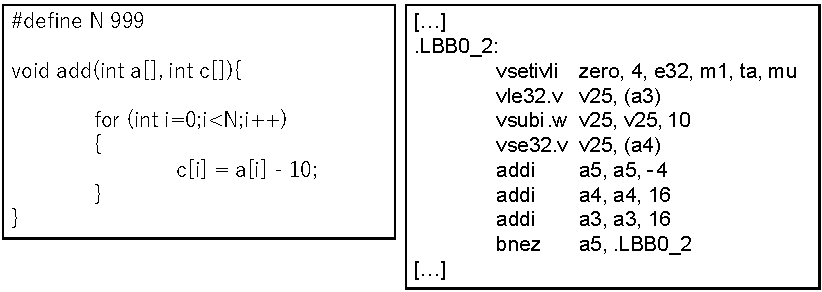
\includegraphics[scale=0.8]{image/vsubi.pdf}
    \caption{vsubi命令の生成}
    \label{fig:vsubi}
\end{figure}

\begin{figure}
    \centering
    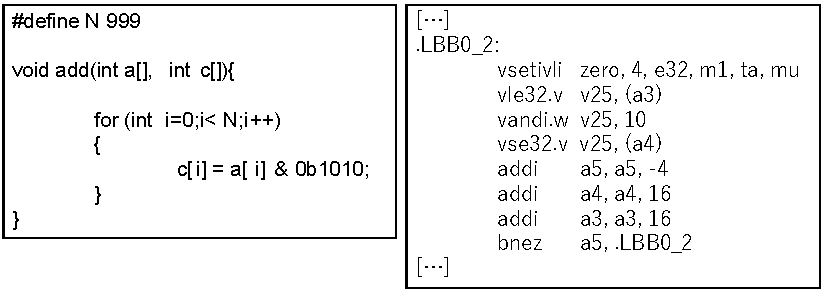
\includegraphics[scale=0.8]{image/vandi.pdf}
    \caption{vandi命令の生成}
    \label{fig:vandi}
\end{figure}

\begin{figure}
    \centering
    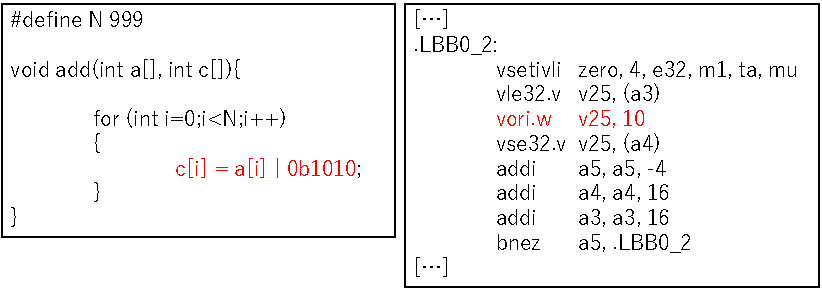
\includegraphics[scale=0.8]{image/vori.pdf}
    \caption{vori命令の生成}
    \label{fig:vori}
\end{figure}

\begin{figure}
    \centering
    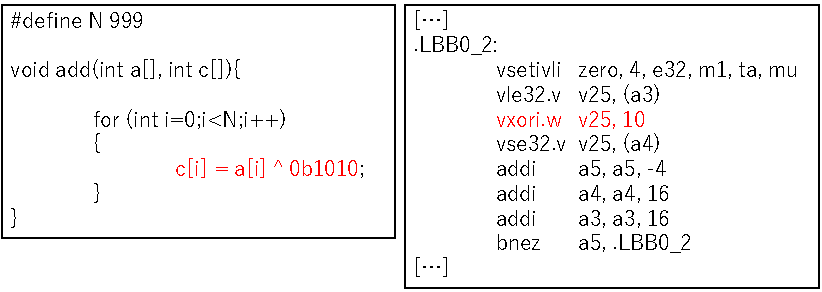
\includegraphics[scale=0.8]{image/vxori.pdf}
    \caption{vxori命令の生成}
    \label{fig:vxori}
\end{figure}

\begin{figure}
    \centering
    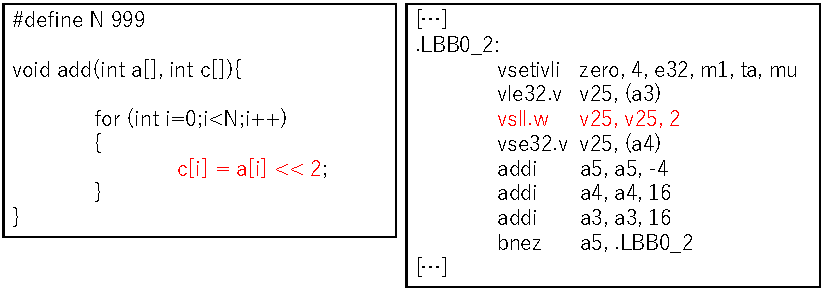
\includegraphics[scale=0.8]{image/vsll.pdf}
    \caption{vsll命令の生成}
    \label{fig:vsll}
\end{figure}

\begin{figure}
    \centering
    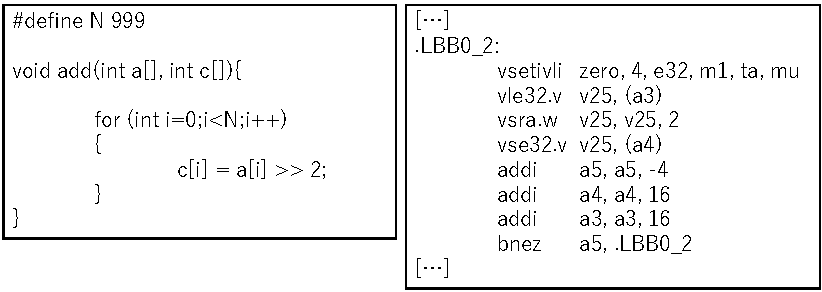
\includegraphics[scale=0.8]{image/vsra.pdf}
    \caption{vsra命令の生成}
    \label{fig:vsra}
\end{figure}

\begin{figure}
    \centering
    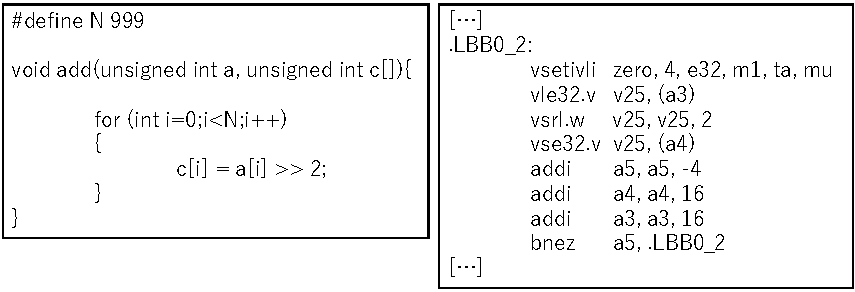
\includegraphics[scale=0.8]{image/vsrl.pdf}
    \caption{vsrl命令の生成}
    \label{fig:vsrl}
\end{figure}